\let\negmedspace\undefined 
 \let\negthickspace\undefined 
 \documentclass[journal,12pt,onecolumn]{IEEEtran} 
 %\documentclass[conference]{IEEEtran} 
 %\IEEEoverridecommandlockouts 
 % The preceding line is only needed to identify funding in the first footnote. If that is unneeded, please comment it out. 
 \usepackage{cite} 
 \usepackage{amsmath,amssymb,amsfonts,amsthm} 
 \usepackage{algorithmic} 
 \usepackage{graphicx} 
 \usepackage{textcomp} 
 \usepackage{xcolor} 
 \usepackage{txfonts} 
 \usepackage{listings} 
 \usepackage{enumitem} 
 \usepackage{mathtools} 
 \usepackage{gensymb} 
 \usepackage[breaklinks=true]{hyperref} 
 \usepackage{tkz-euclide} % loads  TikZ and tkz-base 
 \usepackage{listings} 
 \usepackage{caption}
 % 
 %\usepackage{setspace} 
 %\usepackage{gensymb} 
 %\doublespacing 
 %\singlespacing 
  
 %\usepackage{graphicx} 
 %\usepackage{amssymb} 
 %\usepackage{relsize} 
  %\usepackage[cmex10]{amsmath} 
 %\usepackage{amsthm} 
 %\interdisplaylinepenalty=2500 
 %\savesymbol{iint} 
 %\usepackage{txfonts} 
 %\restoresymbol{TXF}{iint} 
 %\usepackage{wasysym} 
 %\usepackage{amsthm} 
 %\usepackage{iithtlc} 
 %\usepackage{mathrsfs} 
 %\usepackage{txfonts} 
 %\usepackage{stfloats} 
 %\usepackage{bm} 
 %\usepackage{cite} 
 %\usepackage{cases} 
 %\usepackage{subfig} 
 %\usepackage{xtab} 
 %\usepackage{longtable} 
 %\usepackage{multirow} 
 %\usepackage{algorithm} 
 %\usepackage{algpseudocode} 
 %\usepackage{enumitem} 
 %\usepackage{mathtools} 
 %\usepackage{tikz} 
 %\usepackage{circuitikz} 
 %\usepackage{verbatim} 
 %\usepackage{tfrupee} 
 %\usepackage{stmaryrd} 
 %\usetkzobj{all} 
 %    \usepackage{color}                                            %% 
 %    \usepackage{array}                                            %% 
 %    \usepackage{longtable}                                        %% 
 %    \usepackage{calc}                                             %% 
 %    \usepackage{multirow}                                         %% 
 %    \usepackage{hhline}                                           %% 
 %    \usepackage{ifthen}                                           %% 
   %optionally (for landscape tables embedded in another document): %% 
 %    \usepackage{lscape}      
 %\usepackage{multicol} 
 %\usepackage{chngcntr} 
 %\usepackage{enumerate} 
  
 %\usepackage{wasysym} 
 %\newcounter{MYtempeqncnt} 
 \DeclareMathOperator*{\Res}{Res} 
 %\renewcommand{\baselinestretch}{2} 
 \renewcommand\thesection{\arabic{section}} 
 \renewcommand\thesubsection{\thesection.\arabic{subsection}} 
 \renewcommand\thesubsubsection{\thesubsection.\arabic{subsubsection}} 
  
 \renewcommand\thesectiondis{\arabic{section}} 
 \renewcommand\thesubsectiondis{\thesectiondis.\arabic{subsection}} 
 \renewcommand\thesubsubsectiondis{\thesubsectiondis.\arabic{subsubsection}} 
  
 % correct bad hyphenation here 
 \hyphenation{op-tical net-works semi-conduc-tor} 
 \def\inputGnumericTable{}                                 %% 
  
 \lstset{ 
 %language=C, 
 frame=single,  
 breaklines=true, 
 columns=fullflexible 
 } 
 %\lstset{ 
 %language=tex, 
 %frame=single,  
 %breaklines=true 
 %} 
  
 \begin{document} 
 % 
  
  
 \newtheorem{theorem}{Theorem}[section] 
 \newtheorem{problem}{Problem} 
 \newtheorem{proposition}{Proposition}[section] 
 \newtheorem{lemma}{Lemma}[section] 
 \newtheorem{corollary}[theorem]{Corollary} 
 \newtheorem{example}{Example}[section] 
 \newtheorem{definition}[problem]{Definition} 
 %\newtheorem{thm}{Theorem}[section]  
 %\newtheorem{defn}[thm]{Definition} 
 %\newtheorem{algorithm}{Algorithm}[section] 
 %\newtheorem{cor}{Corollary} 
 \newcommand{\BEQA}{\begin{eqnarray}} 
 \newcommand{\EEQA}{\end{eqnarray}} 
 \newcommand{\define}{\stackrel{\triangle}{=}} 
  
 \bibliographystyle{IEEEtran} 
 %\bibliographystyle{ieeetr} 
  
  
 \providecommand{\mbf}{\mathbf} 
 \providecommand{\pr}[1]{\ensuremath{\Pr\left(#1\right)}} 
 \providecommand{\qfunc}[1]{\ensuremath{Q\left(#1\right)}} 
 \providecommand{\sbrak}[1]{\ensuremath{{}\left[#1\right]}} 
 \providecommand{\lsbrak}[1]{\ensuremath{{}\left[#1\right.}} 
 \providecommand{\rsbrak}[1]{\ensuremath{{}\left.#1\right]}} 
 \providecommand{\brak}[1]{\ensuremath{\left(#1\right)}} 
 \providecommand{\lbrak}[1]{\ensuremath{\left(#1\right.}} 
 \providecommand{\rbrak}[1]{\ensuremath{\left.#1\right)}} 
 \providecommand{\cbrak}[1]{\ensuremath{\left\{#1\right\}}} 
 \providecommand{\lcbrak}[1]{\ensuremath{\left\{#1\right.}} 
 \providecommand{\rcbrak}[1]{\ensuremath{\left.#1\right\}}} 
 \theoremstyle{remark} 
 \newtheorem{rem}{Remark} 
 \newcommand{\sgn}{\mathop{\mathrm{sgn}}} 
 \providecommand{\abs}[1]{\left\vert#1\right\vert} 
 \providecommand{\res}[1]{\Res\displaylimits_{#1}}  
 \providecommand{\norm}[1]{\left\lVert#1\right\rVert} 
 %\providecommand{\norm}[1]{\lVert#1\rVert} 
 \providecommand{\mtx}[1]{\mathbf{#1}} 
 \providecommand{\mean}[1]{E\left[ #1 \right]} 
 \providecommand{\fourier}{\overset{\mathcal{F}}{ \rightleftharpoons}} 
 %\providecommand{\hilbert}{\overset{\mathcal{H}}{ \rightleftharpoons}} 
 \providecommand{\system}{\overset{\mathcal{H}}{ \longleftrightarrow}} 
         %\newcommand{\solution}[2]{\textbf{Solution:}{#1}} 
 \newcommand{\solution}{\noindent \textbf{Solution: }} 
 \newcommand{\cosec}{\,\text{cosec}\,} 
 \providecommand{\dec}[2]{\ensuremath{\overset{#1}{\underset{#2}{\gtrless}}}} 
 \newcommand{\myvec}[1]{\ensuremath{\begin{pmatrix}#1\end{pmatrix}}} 
 \newcommand{\mydet}[1]{\ensuremath{\begin{vmatrix}#1\end{vmatrix}}} 
 %\numberwithin{equation}{section} 
 %\numberwithin{equation}{subsection} 
 %\numberwithin{problem}{section} 
 %\numberwithin{definition}{section} 
 %\makeatletter 
 %\@addtoreset{figure}{problem} 
 %\makeatother 
  
 %\let\StandardTheFigure\thefigure 
 \let\vec\mathbf 
 %\renewcommand{\thefigure}{\theproblem.\arabic{figure}} 
 %\renewcommand{\thefigure}{\theproblem} 
 %\setlist[enumerate,1]{before=\renewcommand\theequation{\theenumi.\arabic{equation}} 
 %\counterwithin{equation}{enumi} 
  
  
 %\renewcommand{\theequation}{\arabic{subsection}.\arabic{equation}} 
  
 %\def\putbox#1#2#3{\makebox[0in][l]{\makebox[#1][l]{}\raisebox{\baselineskip}[0in][0in]{\raisebox{#2}[0in][0in]{#3}}}} 
 %     \def\rightbox#1{\makebox[0in][r]{#1}} 
 %     \def\centbox#1{\makebox[0in]{#1}} 
 %     \def\topbox#1{\raisebox{-\baselineskip}[0in][0in]{#1}} 
 %     \def\midbox#1{\raisebox{-0.5\baselineskip}[0in][0in]{#1}} 
  
 \vspace{3cm} 
  
 \title{ Assignment 1 
  
         \Large AI1110: Probability and Random Variables 
  
          INDIAN INSTITUTE OF TECHNOLOGY, HYDERABAD 
 } 
 \author{ LAHARI GUNTI 
          
         AI22BTECH11008 
 } 
  
 \maketitle 
  
 \bigskip 
 \renewcommand{\thefigure}{\theenumi} 
 \renewcommand{\thetable}{\theenumi} 
 \textbf{11.16.3.5}: 
 Given that a fair coin is marked 1 on one face and 6 on the other and a fair die are tossed.find the probability sum turns up to be 3 and 12 \\ 
 \textbf{Solution}: 
         Let the random variable  $X$,$Y$ denote the toss of a coin and roll of a dice.
 \begin{enumerate}[label=(\alph*)] 
	 \item   The  generating function of $X$ is  
                         \begin{align} 
				 M_X(z) &= E\sbrak{z^{-X}} 
				 = \sum_{n=-\infty}^{\infty}p_X\brak{n}z^{-n}  
                         \end{align} 
		 \item Let us define a random variable $Z$,Let X and Y are independent random variables then 
			 \begin{align}
				 M_Z(z) &= E\sbrak{z^{-(X + Y)}} 
					 = E\sbrak{e^{-X}e^{-Y}} = E\sbrak{z^{-X}}E\sbrak{z^{-Y}} \\
					 = M_X(z)M_Y(z) 
			 \end{align}
			 \item  We have 
                        \begin{align}
                                M_X(z) &= \brak{z^{-1}}\brak{\frac{1}{2}} + \brak{z^{-6}}\brak{\frac{1}{2}} 
                        \end{align}
                         \begin{align}
                                 M_Y(z) &= \frac{z^{-1} + z^{-2} + z^{-3} + z^{-4} + z^{-5} + z^{-6}}{6} 
                         \end{align}
                        \begin{align}
                        M_Z(z) &= \sbrak{\frac{z^{-1} + z^{-6}}{2}}\sbrak{\frac{z^{-1} + z^{-2} + z^{-3} + z^{-4} + z^{-5} + z^{-6}}{6}} \\
                                &= \frac{1}{12}\sbrak{z^{-2} + z^{-3} + z^{-4} + z^{-5} + z^{-6} + z^{-8} + z^{-9} + z^{-10} + z^{-11} + z^{-12}} + \frac{1}{6}\sbrak{z^{-7}}
                        \end{align}

		 \item pmf of $X$,$Y$ and $Z$
			 \begin{align}
				 p_X\brak{n} &= \frac{1}{2} & \text{ for $n = \{1,6\}$} 
			 \end{align}
			 \begin{align}
				 p_Y\brak{n} &= \frac{1}{6} & \text{ for} 1 \leqslant\: n < 7
			 \end{align}
			 \begin{align}
				 p_Z\brak{n} = \begin{cases} \frac{1}{12} & \text{if } 2 \leqslant\: n < 7 , \\ \frac{1}{6} & \text{if $n = 7$,} \\ \frac{1}{12} & \text{if } 8 \leqslant\: n < 13 \end{cases}
			 \end{align}
			 \begin{figure}
				 \captionsetup{width=\columnwidth}
				 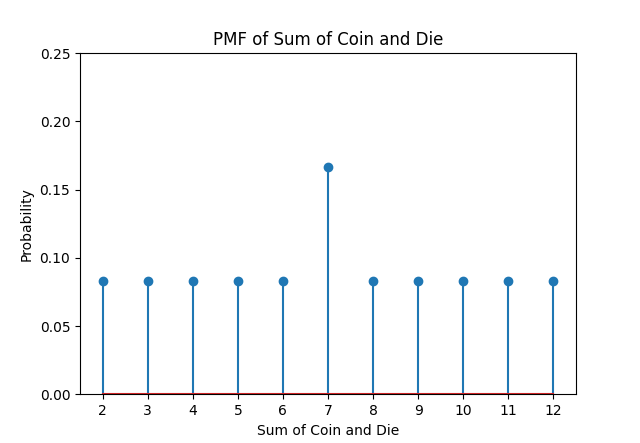
\includegraphics[width=\columnwidth]{1.png}
				 \caption{pmf of the sum when coin and die are rolled simultaneously}
				 \label{fig:pmf}
			 \end{figure}

		 \item from $p_Z\brak{n}$ we get the required probabilities 
	   \begin{align}
		   \pr{Z = 3} &= \frac{1}{12}
	      \end{align}      
              \begin{align}
		      \pr{Z = 12} &= \frac{1}{12}
	      \end{align}
 \end{enumerate} 
 \end{document}
